\documentclass[conference]{IEEEtran}
\IEEEoverridecommandlockouts
% The preceding line is only needed to identify funding in the first footnote. If that is unneeded, please comment it out.
% \usepackage{cite}
\usepackage{url}
\usepackage[english]{babel}
\usepackage{amsmath,amssymb,amsfonts}
\usepackage{algorithmic}
\usepackage{graphicx}
\graphicspath{ {./images/} }
\usepackage{textcomp}
\usepackage{xcolor}
% \def\BibTeX{{\rm B\kern-.05em{\sc i\kern-.025em b}\kern-.08em
%     T\kern-.1667em\lower.7ex\hbox{E}\kern-.125emX}}
\usepackage[sorting=none]{biblatex}
\addbibresource{biblio.bib}

% \def\thesection{\arabic{section}}

\begin{document}

\title{Assignment for the course \\Automated Planning Theory and Practice\\
% {\footnotesize \textsuperscript{*}Note: Sub-titles are not captured in Xplore and
% should not be used}
% \thanks{Identify applicable funding agency here. If none, delete this.}
}

\author{\IEEEauthorblockN{Davide Lusuardi}
\IEEEauthorblockA{\textit{Department of information engineering and computer science} \\
\textit{University of Trento}\\
Trento, Italy \\
davide.lusuardi@studenti.unitn.it}
}

\maketitle

\begin{abstract}
This report is intended to present and analyze the assignment \cite{assignment} 
for the course \textit{Automated Planning Theory and Practice}
and discuss some design choices regarding its modelling and implementation.

The assignment is inspired by an emergency services logistics scenario where
a set of robotic agents have the task to deliver crates containing emergency 
supplies to some injured people.

The assignment is divided into four subproblems, each building on the previous 
one with increasing complexity.
In the first problem, the robot can pick up and move just one crate at time.
In the second problem, the complexity increases a bit given that the robot
exploits a carrier that can load up to four crates.
In the third problem, it is required to use durative actions in order to assign
reasonable duration to different actions and model which actions can be executed
in parallel.
Lastly, the third problem has to be implemented within the \texttt{PlanSys2} 
framework, executing the plan in a simulated environment.

In this report, we show how these problems can be formalized using the PDDL planning
language and solved by state-of-the-art planners.

\end{abstract}

% \begin{IEEEkeywords}
% component, formatting, style, styling, insert
% \end{IEEEkeywords}

\section{Introduction}
Planning is a branch of Artificial Intelligence that seeks to automate reasoning about
formulating a plan to achieve a given goal in a given situation. 
Planning is a model-based approach: a planning system takes as input a model of the initial state, 
the actions available to change it and the goal conditions, producing as output a plan 
that will reach the goal from the initial situation.

The Planning Domain Definition Language (PDDL) is a formal knowledge representation language 
designed to express planning models. Developed by the planning research community, 
it has become a de-facto standard language of many planning systems.

The purpose of the assignment is two-fold: first, to model the given scenario using the PDDL language 
and find a plan using a state-of-the-art planner; second, leveraging the \texttt{PlanSys2} \cite{PlanSys2} 
infrastructure, to integrate the model within a robotic setting.

ROS2 Planning System, \texttt{PlanSys2} in short, is a framework for symbolic planning that incorporates 
novel approaches for execution on robots working in demanding environments \cite{PlanSys2}.

The proposed scenario is inspired by an emergency services logistic problem:
a number of injured people are situated at known locations and one or more robotic agents
have the task to deliver crates containing emergency supplies to each person. 
The planning system should formulate a plan for the robotic agents in order to deliver all
the crates needed by the injured people.

The document is structured as follows: in Section \ref{sec2},
we explain in details our understanding of the proposed scenario and the four subproblems; 
in Section \ref{sec3}, we describe the design choices and the proposed solutions to solve the problem,
making some assumptions in order to constrain the problem; % TODO: scrivere meglio
in Section \ref{sec4}, we discuss and analyze the achieved results and briefly describe the
content of the submitted archive; in Section \ref{sec5}, we make some conclusions and future 
works are proposed.




\section{Understanding of the problem}
\label{sec2}

The assignment proposes four subproblems within the same scenario, each building on the previous one.

The proposed scenario consists of an emergency situation in which there are a number of injured people 
who need emergency supplies.
% to help delivering them some crates containing
Each injured person is located in a specific place and may need some kinds of emergency supply
(e.g. food, medicine, beverage, ...). There may be more people at the same location and some 
locations may be empty.
Each crate is at a specific location and contains just one specific kind of emergency supply.
Some people may already have some crates and some others may not need any crate.
People don't care which crate exactly they get, only the content type is important.
There can be one or more robotic agents that cooperate in order to deliver crates to people.
Each location is connected to every other location, so the robotic agent can move directly between them.
Initially, the robotic agents and the crates are situated at the depot, where there are not injured people.

The goal consists in deliver all the required crates to injured people.

The above considerations and the goal are common for all the four subproblems that we are going to discuss.

\subsection{Problem 1}
This is the easiest problem.
We have that a single robotic agent is present at the depot.
It can perform the following actions: pick up and load just one crate that is at the same location;
move to another location, moving also the loaded crate if present; 
deliver the loaded crate to a person that is at the same location of the robot.

\subsection{Problem 2}
In this subproblem, the robotic agent can move crates in an different way.
We introduce the concept of carrier that can be loaded with up to a specific number of crates, 
in this case up to four.
This number is problem specific and is modeled in the problem file.
At a specific location, the robot can load the carrier with crates situated in that location and can
deliver loaded crates to people.
The robot can move to another location bringing a carrier with it or not.
% The robotic agent can load the carrier with crates at the same location, can move the carrier to another 
% location and 
% At the location of the robot, it can load some crates on the carrier or deliver some others to people.

The difficult part consists in modeling correctly the carrier and its variable capacity.

\subsection{Problem 3}
In this subproblem, it's required to make use of durative actions.
Reasonable durations should be assigned to actions coherently with their time spans and the possibility 
to execute actions in parallel should be analyzed taking into account real constraints.

\subsection{Problem 4}
In this subproblem, it's required to integrate within the PlanSys2 infrastructure the last subproblem.
% Problem 3 has been integrated within the PlanSys2 infrastructure.
% TODO: spiegare meglio



\section{Design Choices}
\label{sec3}

In this section we discuss some design choices and some assumptions that have been made 
analyzing the scenario and the different subproblems: further assumptions are required 
in order to define better the proposed problem.
% during the implementation of the PDDL domain and problem files.

% We can start 

Each crate can have just one content.
Each person can initially have some crates or none.
Each person can need some emergency supplies of specific content, or can need nothing.
We assume that the need of person of a specific content can be satisfied through the delivering 
to it of just one crate having that content (e.g. if Mario needs food, just one crate containing
food is sufficient, no more).
For this reason, the problem file should be defined in a way that does not introduce any form of inconsistency.
For example, we could have that Mario already have a crate containing food but at the same time he needs food.

We assume that a crate already delivered is no more available (TODO), even if it is redundant.


Initially, we need to consider the main object types used in the proposed scenario.
We can simply spot the following types: robot, person, crate, location, content, 
and, from the Problem 2 on, the assignment introduces the concept of carrier.
Each type can be easily understood without further explanations. 
We can note... TODO

We can now start describing the predicates.
% TODO

\subsection{Problem 1}
In order to model the location of robotic agents, people and crates, appropriates predicates should be defined.
We could simply use just one predicate to express objects location, but we preferred to define a predicate for 
each type of objects to improve clarity. In this way, we have defined the predicates 
\texttt{(robot\_at ?r - robot ?l - location)}, \texttt{(person\_at ?p - person ?l - location)} and 
\texttt{(crate\_at ?c - crate ?l - location)}.



As we have said, people need specific emergency supplies. To model this fact, the predicate
\texttt{(need ?p - person ?co - content)} has been defined. The predicate 
\texttt{(have ?p - person ?co - content)} is used to define that a person has a crate with that content.
In order to know if a crate has already been delivered, the predicate \texttt{(available ?c - crate)}
is used: we assume that when a crate is delivered is no more available to be picked up or moved.
TODO: non assumere ciò sarebbe inutile


To model that a robot can be empty or can hold a crate, the predicates \texttt{(empty ?r - robot)} and
\texttt{(hold ?r - robot ?c - crate)} are respectively used.
We note that the predicate \texttt{empty} is not strictly required but it is useful to simplify the modeling
and increase efficiency of the planner.




We can now start describing the actions. Three different actions have been modeled: \texttt{pick\_up}, 
\texttt{move} and \texttt{deliver}.

The action \texttt{pick\_up}, as the name suggests, models the robot that picks up a crate:
the robot and the crate should be at the same location, the robot should be empty and the crate available.

The action \texttt{move} indicates the movement of the robot from one location to another.

The action \texttt{deliver} indicates the delivering of a crate to a person: the person should need emergency
supplies of the same type of the content of the crate, the robot holds the crate and it is at the same location
of the person.


From Problem 2 on, the introduction of the carrier, poses the need to change a bit the model 
introducing the \texttt{carrier} type and the \texttt{(carrier\_at ?ca - carrier ?l - location)} predicate.
Instead, the predicates \texttt{hold} and \texttt{empty} have been removed in favor of the predicate
\texttt{(load ?ca - carrier ?c - crate)} which indicates that the crate is loaded into the carrier.
In order to model the variable capacity of the carriers, the function \texttt{(capacity ?ca - carrier) - number}
has been defined: the function is used to check to remaining capacity of a carrier before load a crate.
The action \texttt{move\_carrier} has also been added and indicates the robot that moves a carrier.

In Problem 3, the actions have been transformed in durative actions, specifying appropriate durations.
A new predicate \texttt{(busy ?r - robot)} has been added in order to model which actions can be executed 
in parallel. 
\section{Results}
\label{sec4}
In this section, we present and analyze the obtained results regarding the execution of the planners on 
the PDDL files.

The submitted archive contains the solutions to the presented problems and it is organized as follows.
We have created four folders, one for each problem, that contain the PDDL domain files and one or more 
PDDL problem files. For each problem file, the plan found by the planner is reported in a separate file.
For \textit{Problem 4}, there is a folder that contains all the code required to execute the \texttt{PlanSys2} 
problem.
% For each problem there is a folder that contains the PDDL domain file and one or more PDDL problem files.
% the plan obtained running the planner on each problem file is reported in 


\subsection{Problem 1}
For this problem, we have modeled two PDDL problem files with increasing complexity.
The planner used to found the solution is \texttt{Downward} using the option \texttt{--alias lama-first}.

In the first problem modeled, there are 4 people, 5 crates, 4 locations and the planner successfully
found an optimal solution that requires the execution of 15 actions.

The second problem modeled is a bit more complex: the number of objects modeled increase to 8 people, 
8 crates and 5 locations. Also in this case, the planner successfully
found an optimal solution that requires the execution of 27 actions.


\subsection{Problem 2}
For this problem, the planner used is \texttt{Enhsp-2020} that is available in \texttt{Planutils}.

The modeled PDDL problem contains 6 people, 6 crates, 4 locations and just one carrier with capacity 4.
Executing the planner with the option \texttt{-anytime}, it managed to find an optimal solution that 
requires performing 16 actions.

\subsection{Problem 3}
For this problem, the planner used is \texttt{Optic} that is available in \texttt{Planutils}.

It has been decided to model two PDDL problem files.
In the second one, there are two robots and two carriers while in the first one only one of both.
In this way, as previously explained, only in the second problem the actions can be perfomed in parallel.

The planner managed to find a plan of duration 34 seconds for for the first problem and a plan of
duration 24 seconds for the second one.
As can be seen in the second plan, some actions are performed simultaneously as desired.

\subsection{Problem 4}
For this problem, the PDDL domain and problem are the same of \textit{Problem 3}.
The problem is specified using a list of terminal commands accepted by \texttt{PlanSys2}.
These commands are reported in a file located in the directory of \textit{Problem 4}.
% The terminal commands required to specify the problem are the equivalent of the PDDL problem file of the 


\begin{figure}[t]
\centerline{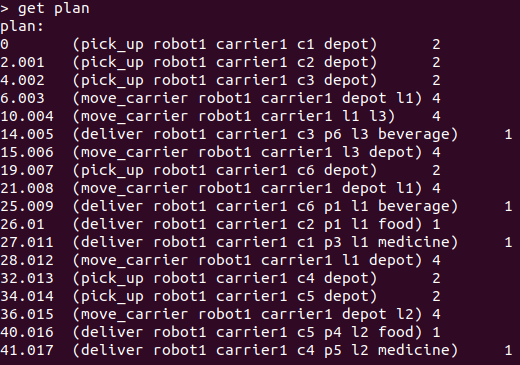
\includegraphics[scale=0.45]{assignment_terminal.png}}
\caption{Plan found by \texttt{POPF} planner.}
\label{fig:plan}
\end{figure}
    
\begin{figure}[t]
\centerline{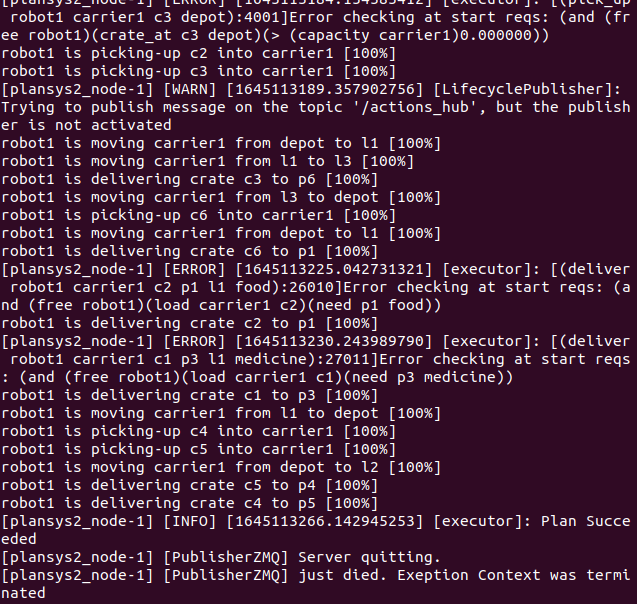
\includegraphics[scale=0.365]{assignment_run.png}}
\caption{\texttt{PlanSys2} execution of the plan.}
\label{fig:execution}
\end{figure}

Executing the \texttt{POPF} planner on this problem, it managed to find the plan shown in Figure 
\ref{fig:plan} of duration 42 seconds.
This plan is then executed by \texttt{PlanSys2} within the \texttt{ROS2} framework. 
Figure \ref{fig:execution} shows part of the execution of the plan and the messages sended by the action nodes.

\section{Conclusions}
\label{sec5}

We have shown how a typical planning problem like the emergency services logistics scenario 
proposed in this report can be solved using the PDDL language and classical planners.

Problems with increasing complexity have been discussed and solved, showing how modern planners can 
efficiently found complex plans.
% This remarks the importance of automated planning for many real applications.

Lastly, we have shown how to integrate the planning problem within the \texttt{PlanSys2} infrastructure
in order to be able to execute the plan in a simulated environment.

In future works, by the use of real robotic agents, it could be interesting to implement real action nodes
and to study the problems that arise in a real environment.

% In future works, it could be interesting use real robotic agents and implement real action nodes in order 
% to solve 





% \bibliographystyle{IEEEtran}
% \bibliography{biblio}

\printbibliography %Prints bibliography

\end{document}